\documentclass[12pt,1in]{article}
\usepackage{amsmath, amssymb}
\usepackage{physics}
\usepackage[margin=1in]{geometry}
\usepackage{cite}
\usepackage{booktabs}
\usepackage{graphicx}
\usepackage{epstopdf}
\usepackage{float}
\usepackage[numbered,framed]{matlab-prettifier}
\newenvironment{Example}[2][Example]{\begin{trivlist}
		\item[\hskip \labelsep {\bfseries #1}\hskip \labelsep {\bfseries #2.}]}{\end{trivlist}}
\usepackage{hyperref}


\lstset{
	caption			   = {MATLAB Source Code},
	style              = Matlab-editor,
	basicstyle         = \tiny\mlttfamily,
	escapechar         = ",
	mlshowsectionrules = true,
	label			   = {lst:source_code}
}

\title{Analyzing Non-linear Ordinary Differential Equations\\ {\small MATH 26600}}
\author{Rutuj Gavankar}
\date{}
\begin{document}

\maketitle

\section{Introduction}

\subsection{Linearizing a system}
A system of linear differential equations is easy to analyze and has analytical solutions in most cases. To analyze as system of non-linear equations, the system must be linearized. 
Let 
\begin{align}
\derivative{x}{t} &= F(x, y) \\
\derivative{y}{t} &= G(x , y)
\end{align}
be a system of first-order differential equations. The steady-state solutions of this system are the solutions for which  $x(t)$ and $y(t)$ are invariant. That is to say,
\begin{align}
    F(x,y) &= 0 \\
    G(x,y) &= 0
\end{align}
We can analyzing this system around these equilibrium points by making linear approximations of the function around these points. Using first order Taylor series expansion for $F$ and $G$ we get
\begin{align}
    F(x,y) &\approx F(x_0, y_0) + F_x(x_0, y_0)(x - x_0) + F_y(x_0, y_0)(y - y_0) \\
    G(x,y) &\approx G(x_0, y_0) + G_x(x_0, y_0)(x - x_0) + G_y(x_0, y_0)(y - y_0)
\end{align}
Where $x_0$ and $y_0$ are the equilibrium points for the system. The system can be re-written in matrix-vector notation as 
\begin{align}
    \begin{bmatrix}
    \derivative{x}{t} \\
    \derivative{y}{t}
    \end{bmatrix} &= 
    \begin{bmatrix}
    F_x(x_0, y_0) & F_y(x_0, y_0)\\
    G_x(x_0, y_0) & G_y(x_0, y_0)
    \end{bmatrix}
    \begin{bmatrix}
    x - x_0 \\
    y - y_0
    \end{bmatrix}
\end{align}Now, let $x - x_0$ be $u$ and $y - y_0$ be $v$, and $\Vec{v}$ be the vector $\left<u ,v\right>$
\begin{align}
    \therefore \derivative{\Vec{v}}{t} &= J\Vec{v} \label{eq:vec_mat}
\end{align}
Where $J$ is the Jacobian matrix, $$J = \begin{bmatrix}
    F_x(x_0, y_0) & F_y(x_0, y_0)\\
    G_x(x_0, y_0) & G_y(x_0, y_0)
    \end{bmatrix}$$
Now, Eq. \ref{eq:vec_mat} is an eigenvalue problem. The local stability and the behaviour of the system around the equilibrium points can be inferred from the eigenvalues of $J$. 

\subsection{Characterizing a system}
Near the equilibrium points, the non-linear system has similar behavior to the linear approximation, and thus, the stability of the system can be analyzed by analyzing the eigenvalues of the system. Let $\lambda_{1,2}$ be the eigenvalues of the system.
\begin{enumerate}
	\item If the eigenvalues of the system are real and positive at an equilibrium point, ($\lambda_{1,2} > 0$), the point is a \emph{nodal-source}. The solutions tend to diverge away from this point. The system is unstable around this point. 
	\item If the eigenvalues of the system are real and negative at an equilibrium point, ($\lambda_{1,2} < 0$),the point is a \emph{nodal-sink}. The solutions tend to converge towards this point. The system is stable around this point. 
	\item If the eigenvalues of the system are real, but $\lambda_1 < 0$ and $\lambda_2 > 0$, the point is a \emph{saddle point}. The solutions tend to diverge away from this point. The system is unstable around this point.
	\item If the eigenvalues of the system imaginary, $(\lambda_{1,2} = \pm k i)$, the point is a \emph{center}.  The solutions tend to oscillate around this point. The system is stable around this point.
	\item If the eigenvalues of the system are complex, $(\lambda_{1,2} = a \pm b i)$, and $\Re{\lambda_{1,2}}> 0$, the point is a \emph{spiral-source}. The solutions tend to spiral-out from the equilibrium point. The system is unstable around this point.
	\item If the eigenvalues of the system are complex, $(\lambda_{1,2} = a \pm b i)$, and $\Re{\lambda_{1,2}}< 0$, the point is a \emph{spiral-source}. The solutions tend to spiral-in to the equilibrium point. The system is stable around this point.
\end{enumerate}

\subsection{Quantitative Analysis of a System}

\subsection{Examples and Solutions}
\begin{Example}{1} \cite[p.~488]{diff_eq}
	Consider the system for $(x,y \geq 0)$
	\begin{align*}
    \derivative{x}{t} &= x(10 - x - y) \\
    \derivative{y}{t} &= y(30 - 2x - y)
\end{align*}
The Jacobian of the system is 
\begin{align*}
    J = \begin{bmatrix}
    10 - 2x - y & -x \\
    -2y & 30 - 2x - 2y
    \end{bmatrix}
\end{align*}
The system has equilibrium points at $(0,0)$, $(10,0)$, $(0,30)$. Analyzing the system at $(0,0)$,
\begin{align*}
    J|_{(0,0)} &= \begin{bmatrix}
    10 & 0 \\
    0 & 30
    \end{bmatrix}
\end{align*}
Since $J$ is a diagonal matrix, the eigenvalues of $J$ are the elements along its diagonal. That is, $\lambda_{1,2} = \{ 10, 30 \}$. Since both the eigenvalues are real and positive, the point $(0,0)$ is a nodal-source.
Similarly, analyzing the system at $(10,0)$,
\begin{align*}
    J|_{(10,0)} &= 
    \begin{bmatrix}
    -10 & -10\\
    0 & 10 
    \end{bmatrix}
\end{align*}
The eigenvalues of $J$ are $\lambda_{1,2} = \{-10, 10\}$. Since both the eigenvalues are real and nonzero, and $\lambda_1 < 0$, $\lambda_2 > 0$, the point $(10,0)$ is a saddle point. 
Now analyzing the system at $(0,30)$,
\begin{align*}
J|_{(0,30)} &= \begin{bmatrix}
-20 & 0 \\
-60 & -30 
\end{bmatrix}
\end{align*}
The eigenvalues for $J$ are $\lambda_{1,2} = \{-30, -20\}$. Since both eigenvalues are real and negative, $(0,30)$ is a nodal-sink. 
Now to graphically analyze the system, the nullclines can be plotted in the phase plane.
To find the $x$-nullclines,
\begin{align*}
\derivative{x}{t} &= 0\\
\therefore x(10 - x -y) &= 0
\end{align*}
That is, $x = 0$ or $y = 10 - x$. 
To find the $y$-nullclines,
\begin{align*}
\derivative{y}{t} &= 0\\
\therefore y(30 - 2x - y) &= 0
\end{align*}
That is, $y = 0$ or $y = 30 - 2x$. 
The nullclines intersect at $(0,0)$, $(10,0)$, $(15,0)$, $(0,30)$, which are the steady-state points of this system. In Fig.\ref{fig:example1} the quantitative analysis of the system can be graphically verified by observing the direction of the vector fields around steady-states. 
The 
\begin{figure}[H]
	\centering
	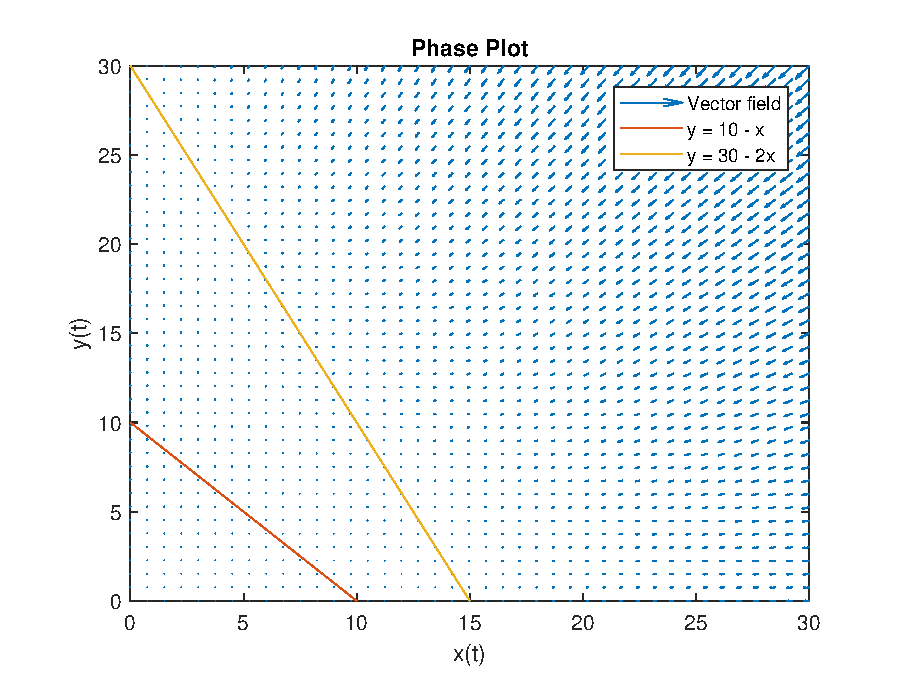
\includegraphics[width=\linewidth,height=.85\linewidth]{Figures/example_1}
	\caption{Nullclines and vector fields}
	\label{fig:example1}
\end{figure}

\end{Example}

\begin{Example}{2}
	\cite[p.~488]{diff_eq}
	Consider the system for $(x,y \geq 0)$
	\begin{align*}
	\derivative{x}{t} &= x(2 - x - y)\\
	\derivative{y}{t} &= y(y - x^2)
	\end{align*}
	The Jacobian of the system is
	\begin{align*}
	J = \begin{bmatrix}
	2 -2x  -y & -x \\
	-2xy & 2y - x^2 
	\end{bmatrix}
	\end{align*}
	Steady-states in the region $(x,y \geq 0)$ are $(0,0)$ , $(1,1)$, and $(2,0)$. Analyzing point $(0,0)$,
	\begin{align*}
	J|_{(0,0)} = \begin{bmatrix}
	2 & 0 \\
	0 & 0
	\end{bmatrix}
	\end{align*}
	The eigenvalues of $J$ are $\lambda_{1,2} = \{2, 0\}$. Since the eigenvalues are non-negative, the solution diverges from $(0,0)$ and the system is unstable around this point. 
	At $(1,1)$
	\begin{align*}
	J|_{(1,1)} &= \begin{bmatrix}
	-1 & -1 \\
	-2 & 1
	\end{bmatrix}
	\end{align*}
	The eigenvalues of $J$ at this point are $\lambda_{1,2} = \pm \sqrt{3}$. Since both the eigenvalues have opposite signs, the point $(1,1)$ is a saddle point, and the system is unstable around this point. At point $(2,0)$,
	\begin{align*} J|_{(2,0)} &=
	\begin{bmatrix}
	-2 & -2 \\
	0 & - 4
	\end{bmatrix}
	\end{align*} 
	The eigenvalues of $J$ at this point are $\lambda_{1,2} = \{-2,-4\}$. Since both the eigenvalues are negative, the point $(2,0)$ is a nodal-sink, and the system is stable around this point. The $x$-nullclines are given by 
	\begin{align*}
	\derivative{x}{t} &= 0 \\
	\therefore x(2 - x - y) &= 0
	\end{align*}
	That is, $x = 0$ and $y = 2 - x$. The $y$-nullclines are given by 
	\begin{align*}
	\derivative{y}{t} &= 0\\
	\therefore y(y - x^2 ) &= 0
	\end{align*}
	That is, $y = 0$ and $y = x^2$. The $x$ and $y$ nullclines intersect at $(0,0)$, $(1,1)$ and $(2,0)$, which are the steady-states of the system for $(x,y \ge 0)$. Fig.\ref{fig:example2} shows the vector field and $xy$ nullclines on the phase plane. 
\begin{figure}[H]
	\centering
	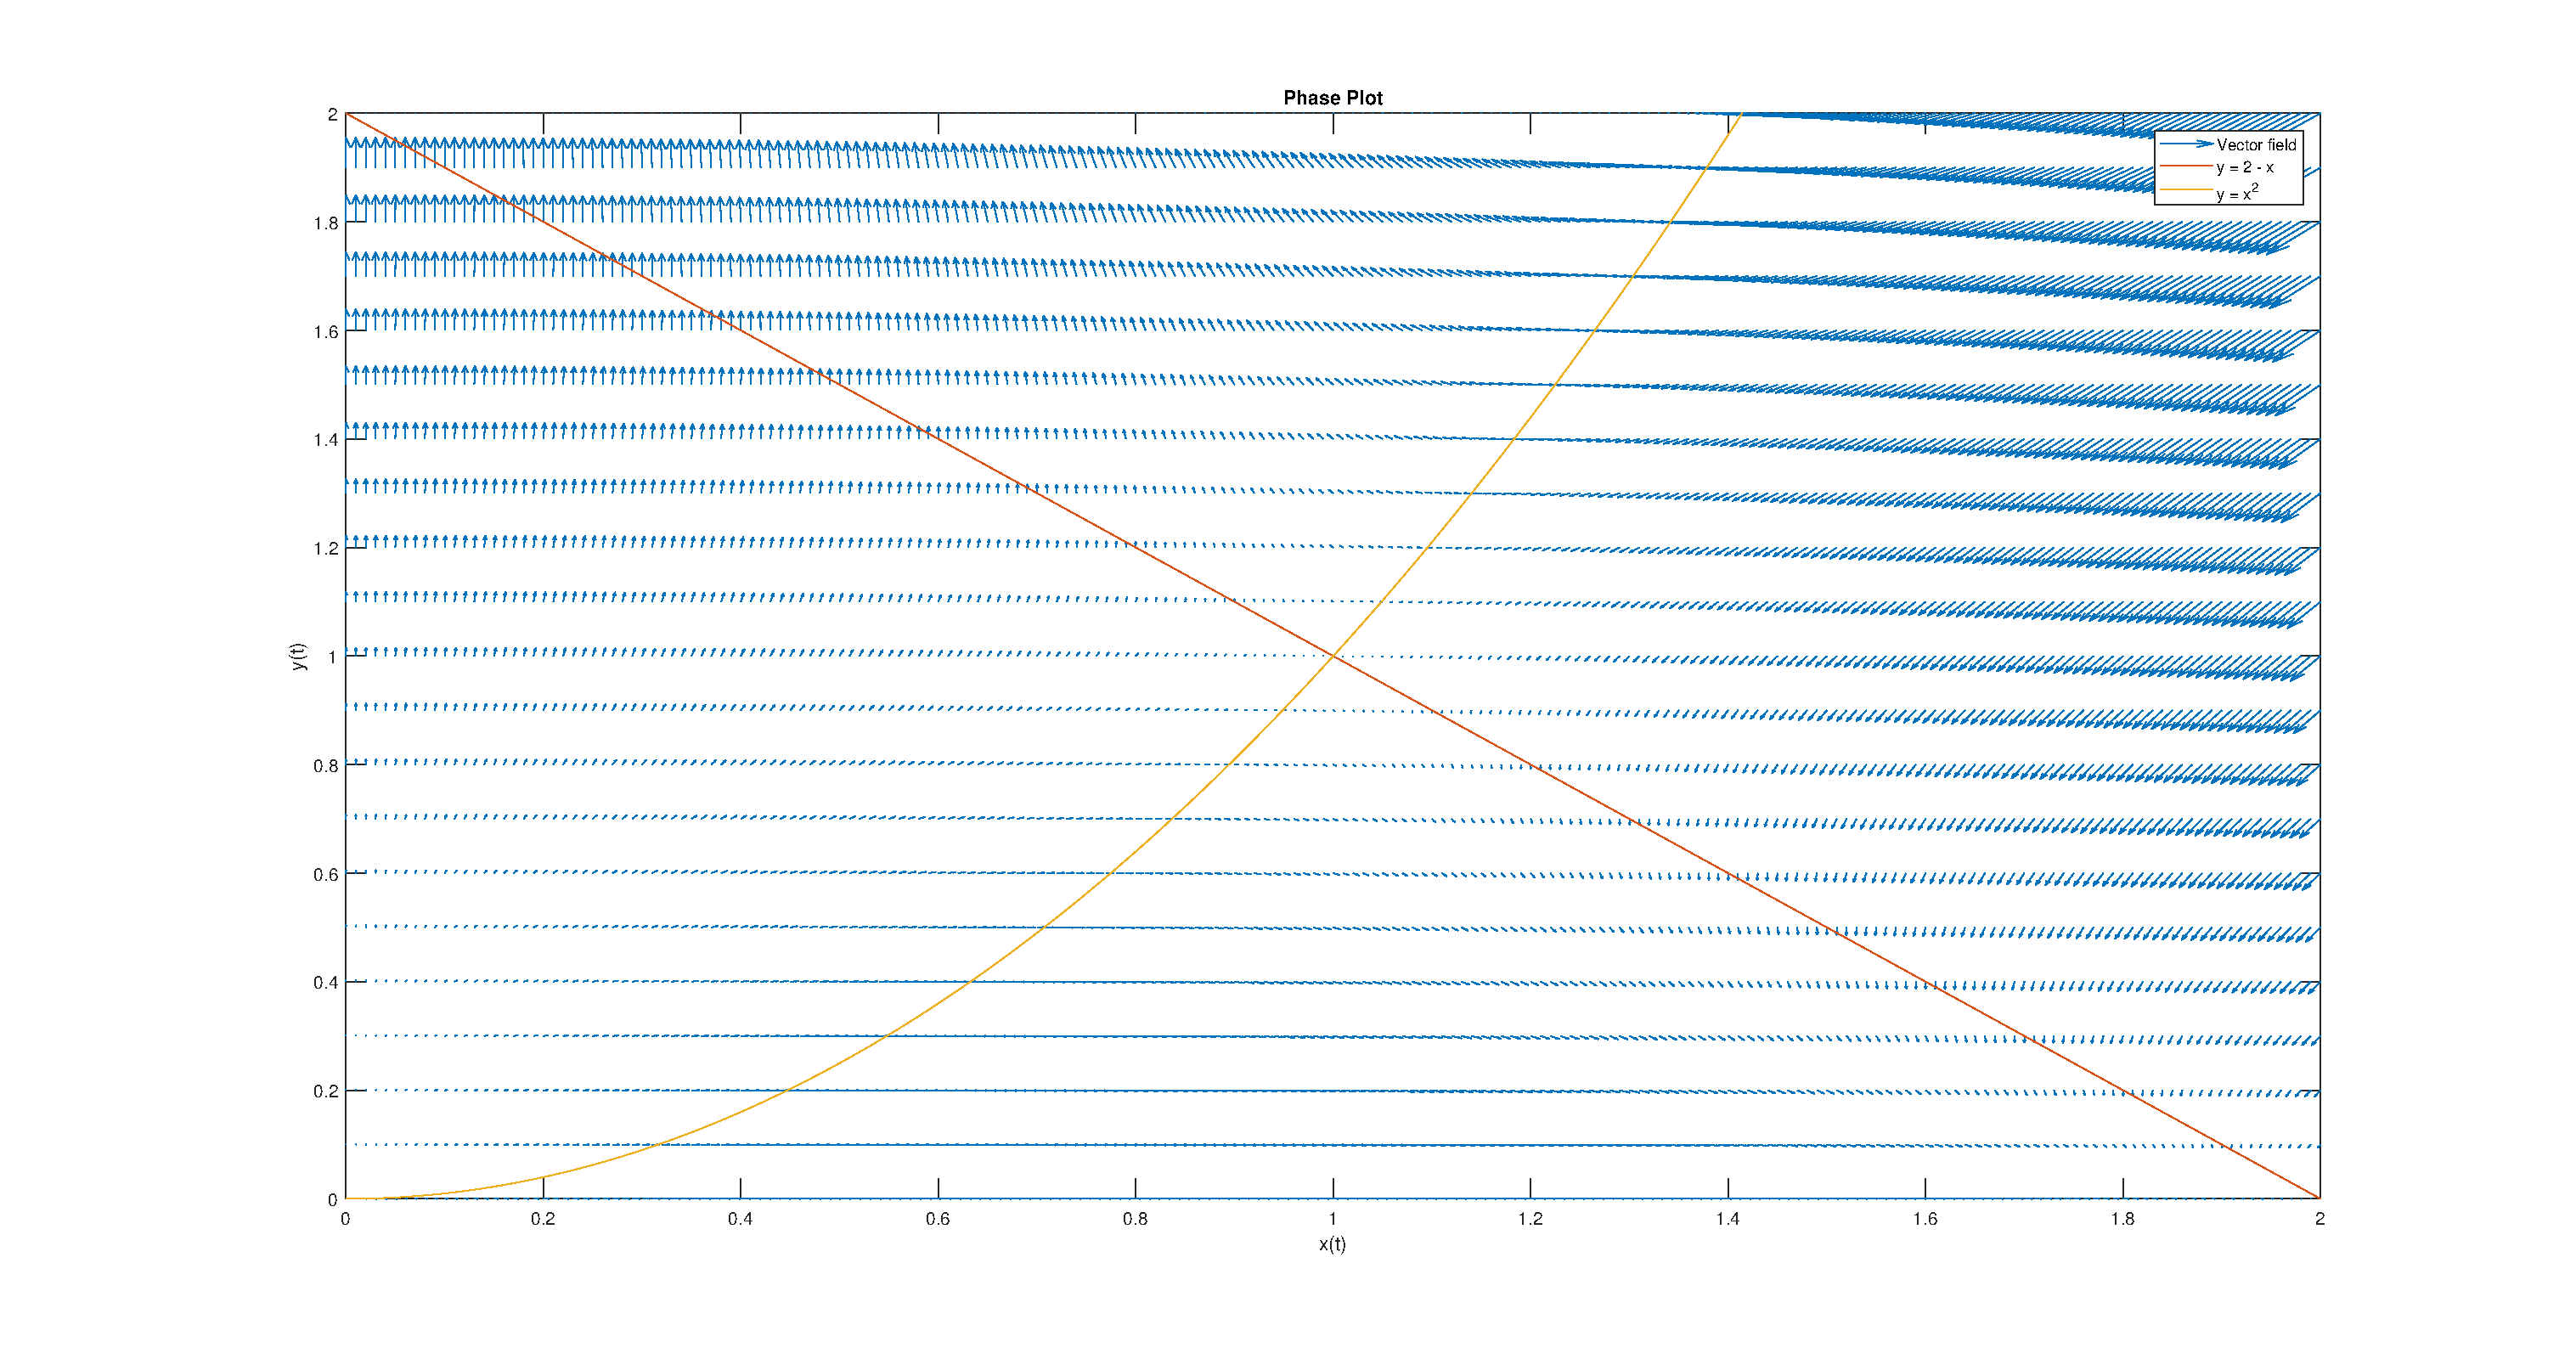
\includegraphics[trim={2in 0 2in 0},width=\linewidth]{Figures/example_2}
	\caption{Nullclines and vector fields}
	\label{fig:example2}
\end{figure}
\end{Example}
\begin{Example}{3}
	\cite[p.~487]{diff_eq}
	\begin{align*}
	\derivative{x}{t} &= x(x - 1)\\
	\derivative{y}{t} &= x^2 - y
	\end{align*}
	For 
	\begin{enumerate}
		\item $x_0 = -1$, $y_0 = 0$
		\item $x_0 = 0.8$, $y_0 = 0$
		\item $x_0 = 1$, $y_0 = 3$
	\end{enumerate}
\begin{figure}[H]
	\centering
	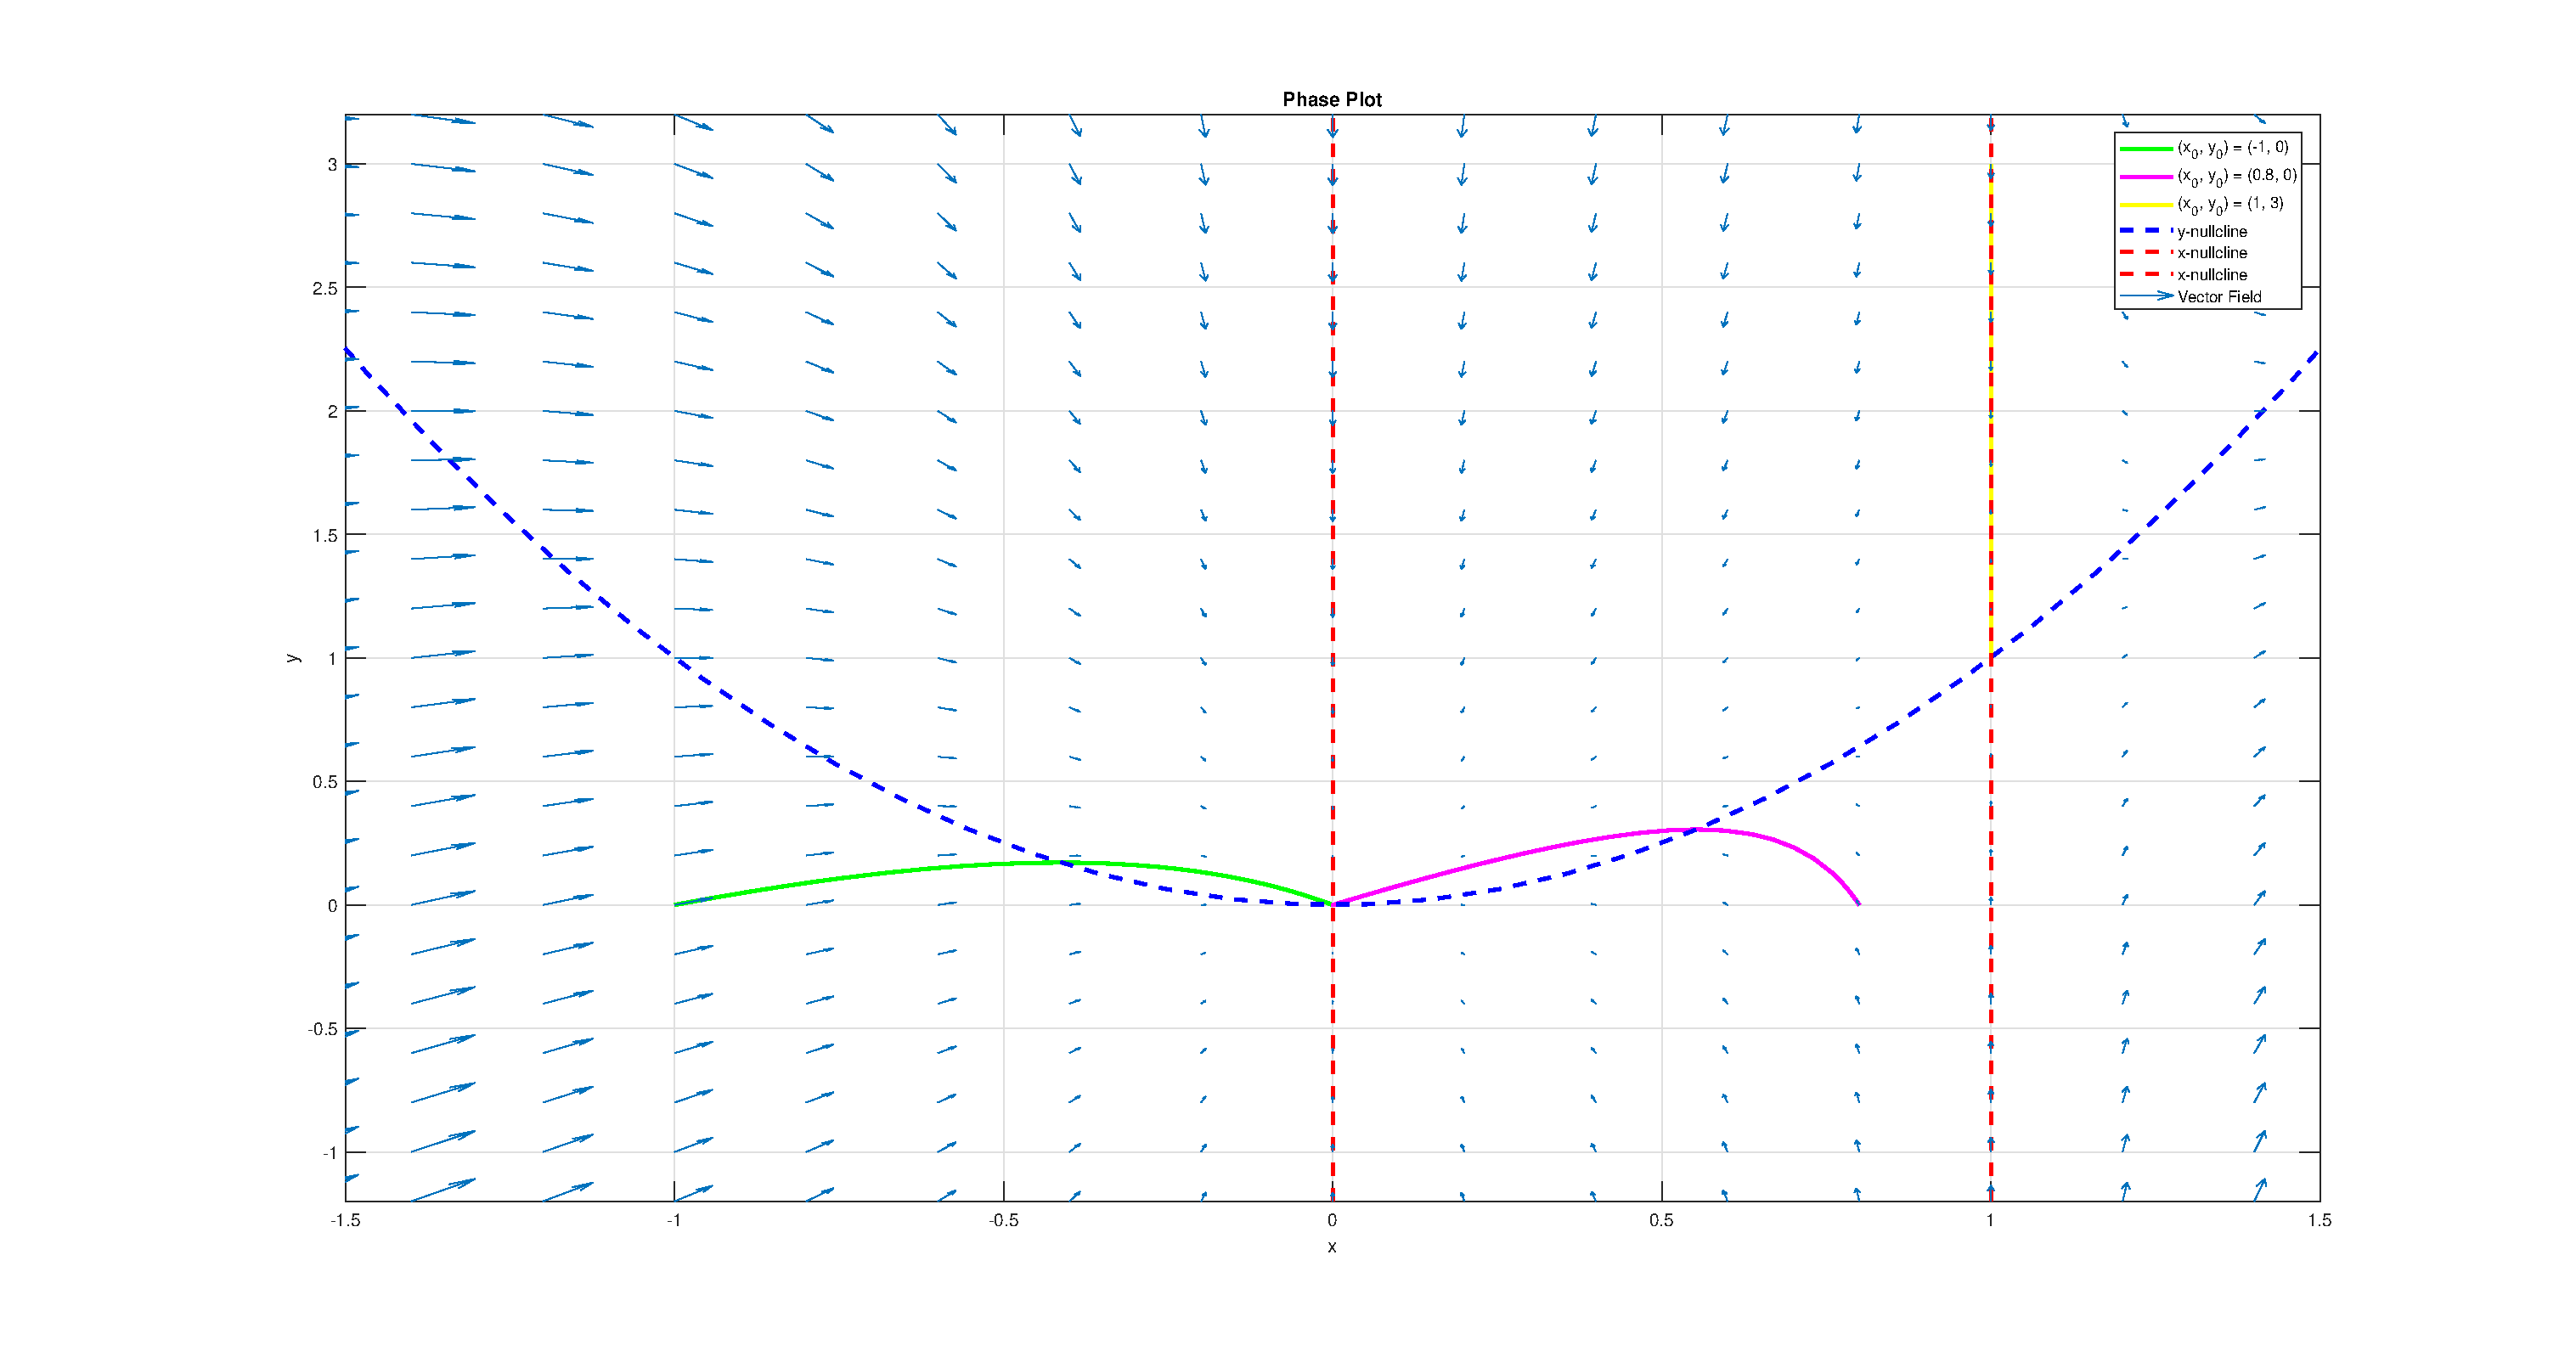
\includegraphics[trim={2in 0 2in 0},width=1\linewidth]{Figures/example_3_phase}
	\caption{Solution Curves and Nullclines}
	\label{fig:example3}
\end{figure}
Figure \ref{fig:example3} shows the solution curves in the $xy$-plane with $t$ as an implicit parameter. The direction of the arrows shows the tendancy of the solutions as $t\rightarrow\infty$. The above system has $x$-nullclines at $x = 0$ and $x = 1$ and $y$-nullclines at $y = x^2$. The interesection points of the nullclines are the steady-states of the system. The MATLAB source code for the generated plots can be found in Listing \ref{lst:source_code}
 
\end{Example}
\section{Hamiltonian Systems}
\subsection{Conserved Quantities and Hamiltonians}
A real-valued function $H(x,y)$ is a \textit{conserved quantity} if
\begin{align}
\derivative{}{t}H(x(t), y(t) = 0
\end{align}
A system of differential equations is called a \textit{Hamiltonian system} if there exists a real-valued function $H(x,y)$ such that 
\begin{align}
\derivative{x}{t} &= \frac{\partial H}{\partial y} \label{ham_1} \\
\derivative{y}{t} &= - \frac{\partial H}{\partial x} \label{ham_2}
\end{align}
\subsection{Characterizing a Hamiltonian system}
The Jacobian of such a system is given by 
\begin{align}
J &= \begin{bmatrix}
\frac{\partial^2H}{\partial x \partial y} & \frac{\partial^2H}{\partial y^2} \\
\frac{\partial^2H}{\partial x^2} & -\frac{\partial^2H}{\partial x \partial y}
\end{bmatrix} \\
&= \begin{bmatrix}
\alpha & \beta \\
\gamma & -\alpha
\end{bmatrix}
\end{align}
The eigenvalues of the matrix $J$ are $\lambda_{1,2} = \pm \sqrt{\alpha^2 + \beta\lambda}$. Now,
\begin{enumerate}
	\item If $\alpha^2 + \beta\lambda > 0$, both eigenvalues will be real and have opposite signs, and equilibrium point will be a saddle. 
	\item If $\alpha^2 + \beta\lambda < 0$, both eigenvalues are imaginary and complex-conjugates. The equilibrium  point will be a center. 
	\item If $\alpha^2 + \beta\lambda = 0$, the only eigenvalue is $\lambda = 0$. This test is inconclusive and requires further analysis, but since the system is Hamiltonian, the equilibrium point cannot be a source or a sink \cite{diff_eq}.  
\end{enumerate}
\subsection{Constructing the Hamiltonian function \label{sec:constructing_hamiltonian}}
If a system 
\begin{align}
x'(t) &= f(x,y) \\
y'(t) &= g(x,y)
\end{align}
is Hamiltonian, with an unknown Hamiltonian function $H(x,y)$ then, \cite{diff_eq}
\begin{align}
\frac{\partial f}{\partial x} &= -\frac{\partial g}{\partial y}  \\
f(x,y) &= \frac{\partial H}{\partial y} \\
g(x,y) &=  - \frac{\partial H}{\partial x}
\end{align}
That is,
\begin{align}
H(x,y) &= \int f(x,y) \dd{y} + \phi(x)
\end{align}
where $\phi(x)$ is a scalar function that is independent of $y$. That is,
\begin{align}
\phi'(x) = - g ( x , y ) - \frac { \partial } { \partial x } \int f ( x , y ) \dd{y}
\end{align}
Thus the Hamiltonian function can be constructed by 
\begin{align}
H(x,y) &= \int f(x,y) \dd{y} + \int \phi'(x) \dd{x}
\end{align}
\subsection{Applications of Hamiltonian Systems - Non-linear Pendulum}
For an ideal-pendulum with mass $m = 1$, length $l = 1$ and no friction, the system describing the motion in polar coordinates is 
\begin{align}
\derivative{\theta}{t} &= \omega \\
\derivative{\omega}{t} &= -g \sin\theta
\end{align}  
where $\theta$ is the angular displacement and $\omega$ is the angular velocity of the pendulum. 

The system has periodic steady-states at $(\theta, \omega ) = (n\pi , 0)$ where $n = 0,1,2,\ldots$. Physically, since there is no friction in the system, the total energy has to be conserved at every point in the system, implying that the total energy of the system is the Hamiltonian function for the system. The total energy for the system at any point in space and time is the total kinetic energy $T$ and the total potential energy $U$. The Hamiltonian can be constructed by $H(\theta, \omega, t) = T(\omega, t) + U(\theta, t)$ \cite{engr_math}. That is,
\begin{align}
H(\theta,\omega, t) &= \frac{m l^2 \omega^2}{2} + mgl(1 - \cos\theta) \\
&= \frac{\omega^2}{2} - g\cos\theta
\end{align}
since $m,l = 1$ and $g$ is a constant. Alternatively, the Hamiltonian can be formulated by the method in Section \ref{sec:constructing_hamiltonian}. 

As seen in Figure \ref{fig:pendulum_phase} and Figure \ref{fig:pendulum_solution_curves}, the solution curves depend on the initial conditions. If the initial angle $\theta$ is an integer multiple of $\pi$, and the initial velocity is $0$, the 
\begin{figure}[H]
	\centering
	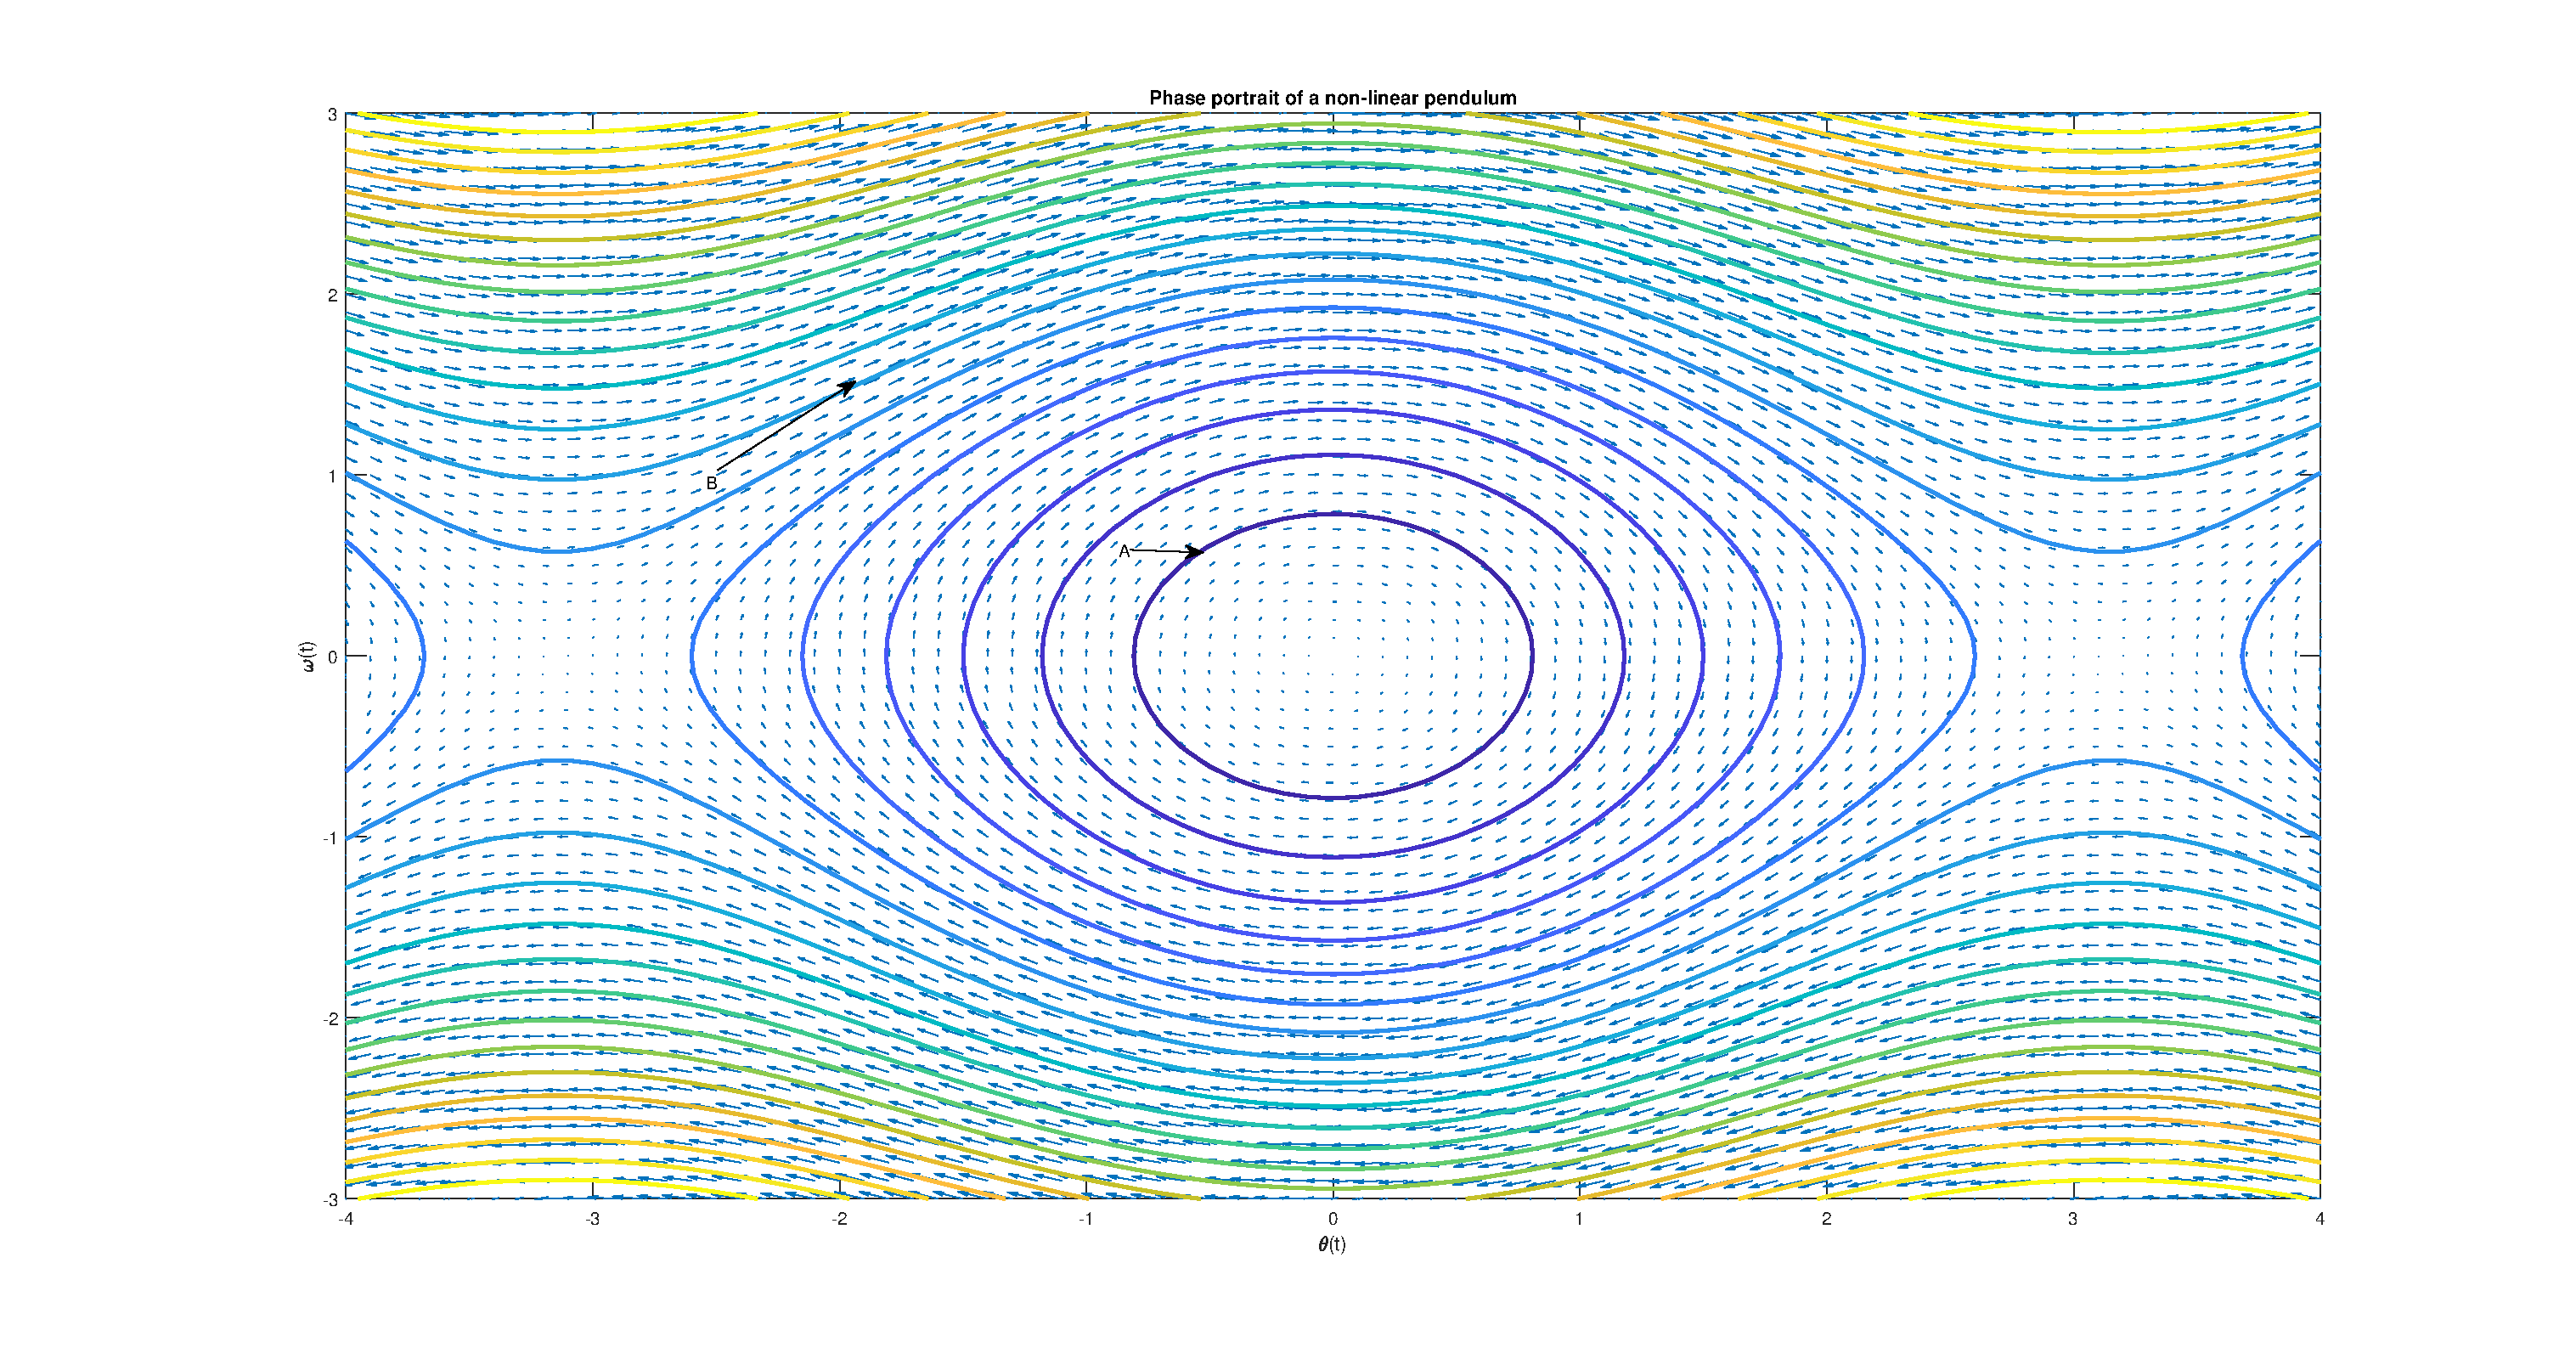
\includegraphics[trim={2in 0 1.5in 0}, width=\linewidth]{Figures/pendulum_phase}
	\caption{Phase portrait of a non-linear pendulum}
	\label{fig:pendulum_phase}
\end{figure}

\begin{figure}[H]
	\centering
	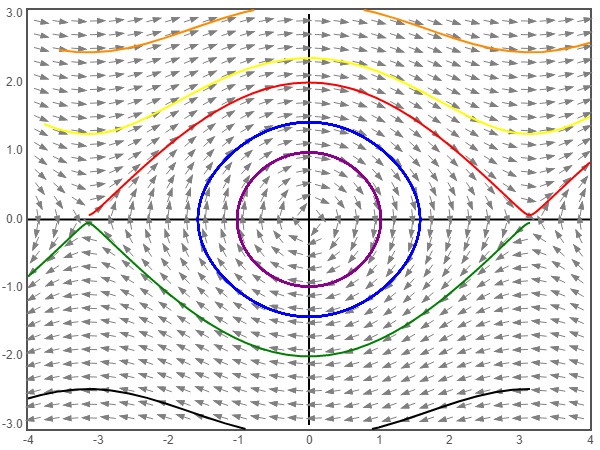
\includegraphics[width=0.7\linewidth]{Figures/phase_online_pendulum}
	\caption{Solution Curves for an ideal-pendulum with different initial conditions}
	\label{fig:pendulum_solution_curves}
\end{figure}

\subsection{Examples}
\begin{Example}{1}
	\begin{align*}
	\derivative{x}{t} &= y \\
	\derivative{y}{t} &= x^2 - a
	\end{align*}
	Where $a$ is a parameter. \\
	{\bfseries Solution\\}
	\begin{align*}
	H(x,y) &= \frac{y^2}{2} - \frac{x^3}{3} + ax
	\end{align*}
	To verify that this system is a Hamiltonian system if $H$ is the Hamiltonian function,
	\begin{align*}
	\frac{\partial}{\partial y}H(x,y) &= y\\
	&= \derivative{x}{t}
	\end{align*}
	and,
	\begin{align*}
	- \frac{\partial}{\partial x} H(x,y) &= x^2 - a\\
	&= \derivative{y}{t}
	\end{align*}
	Since $H_x(x,y) = - y'(t)$ and $H_y(x,y) = x'(t)$, the system is Hamiltonian for $H(x,y)$ as the Hamiltonian function (From Eq. \ref{ham_1} and Eq. \ref{ham_2}).
	
	
	The $x$-nullcline for the system is given by $\derivative{x}{t} = 0$, that is, $y = 0$ and the $y$-nullcline is given by $\derivative{y}{t}=0$, that is, $(x -a)(x+a) = 0$. The intersection of these nullclines is the equilbrium point of the system. So, the equilbrium points of the system are at $(\pm\sqrt{a}, 0)$ if $a > 0$ and no equilbrium points if $a < 0$ ($\because x \in \Im$).
	
	The Jacobian of the above system is given by 
	\begin{align*}
	J = \begin{bmatrix}
	0 & 1 \\
	2x & 0
	\end{bmatrix}
	\end{align*} 
	At the equilibrium point $(\sqrt{a}, 0)$, the Jacobian is 
	\begin{align*}
	J &= \begin{bmatrix}
	0 & 1 \\
	2\sqrt{a} & 0
	\end{bmatrix}
	\end{align*}
	and the eigenvalues of the system at this point are $\lambda_{1,2} = \pm \sqrt{2 \sqrt{a}}$. Since both the eigenvalues have opposite signs, the point $(\sqrt{a}, 0)$ is a saddle point and the system is asymptomatically unstable around this point. At the point $(-\sqrt{a}, 0)$, the Jacobian is 
	\begin{align*}
	J = \begin{bmatrix}
	0 & 1 \\
	-2\sqrt{a} & 0
	\end{bmatrix}
	\end{align*} 
	and the eigenvalues of the system at this point are $\lambda_{1,2} = \pm i \sqrt{2 \sqrt{a}}$
	
\begin{figure}[H]
	\centering
	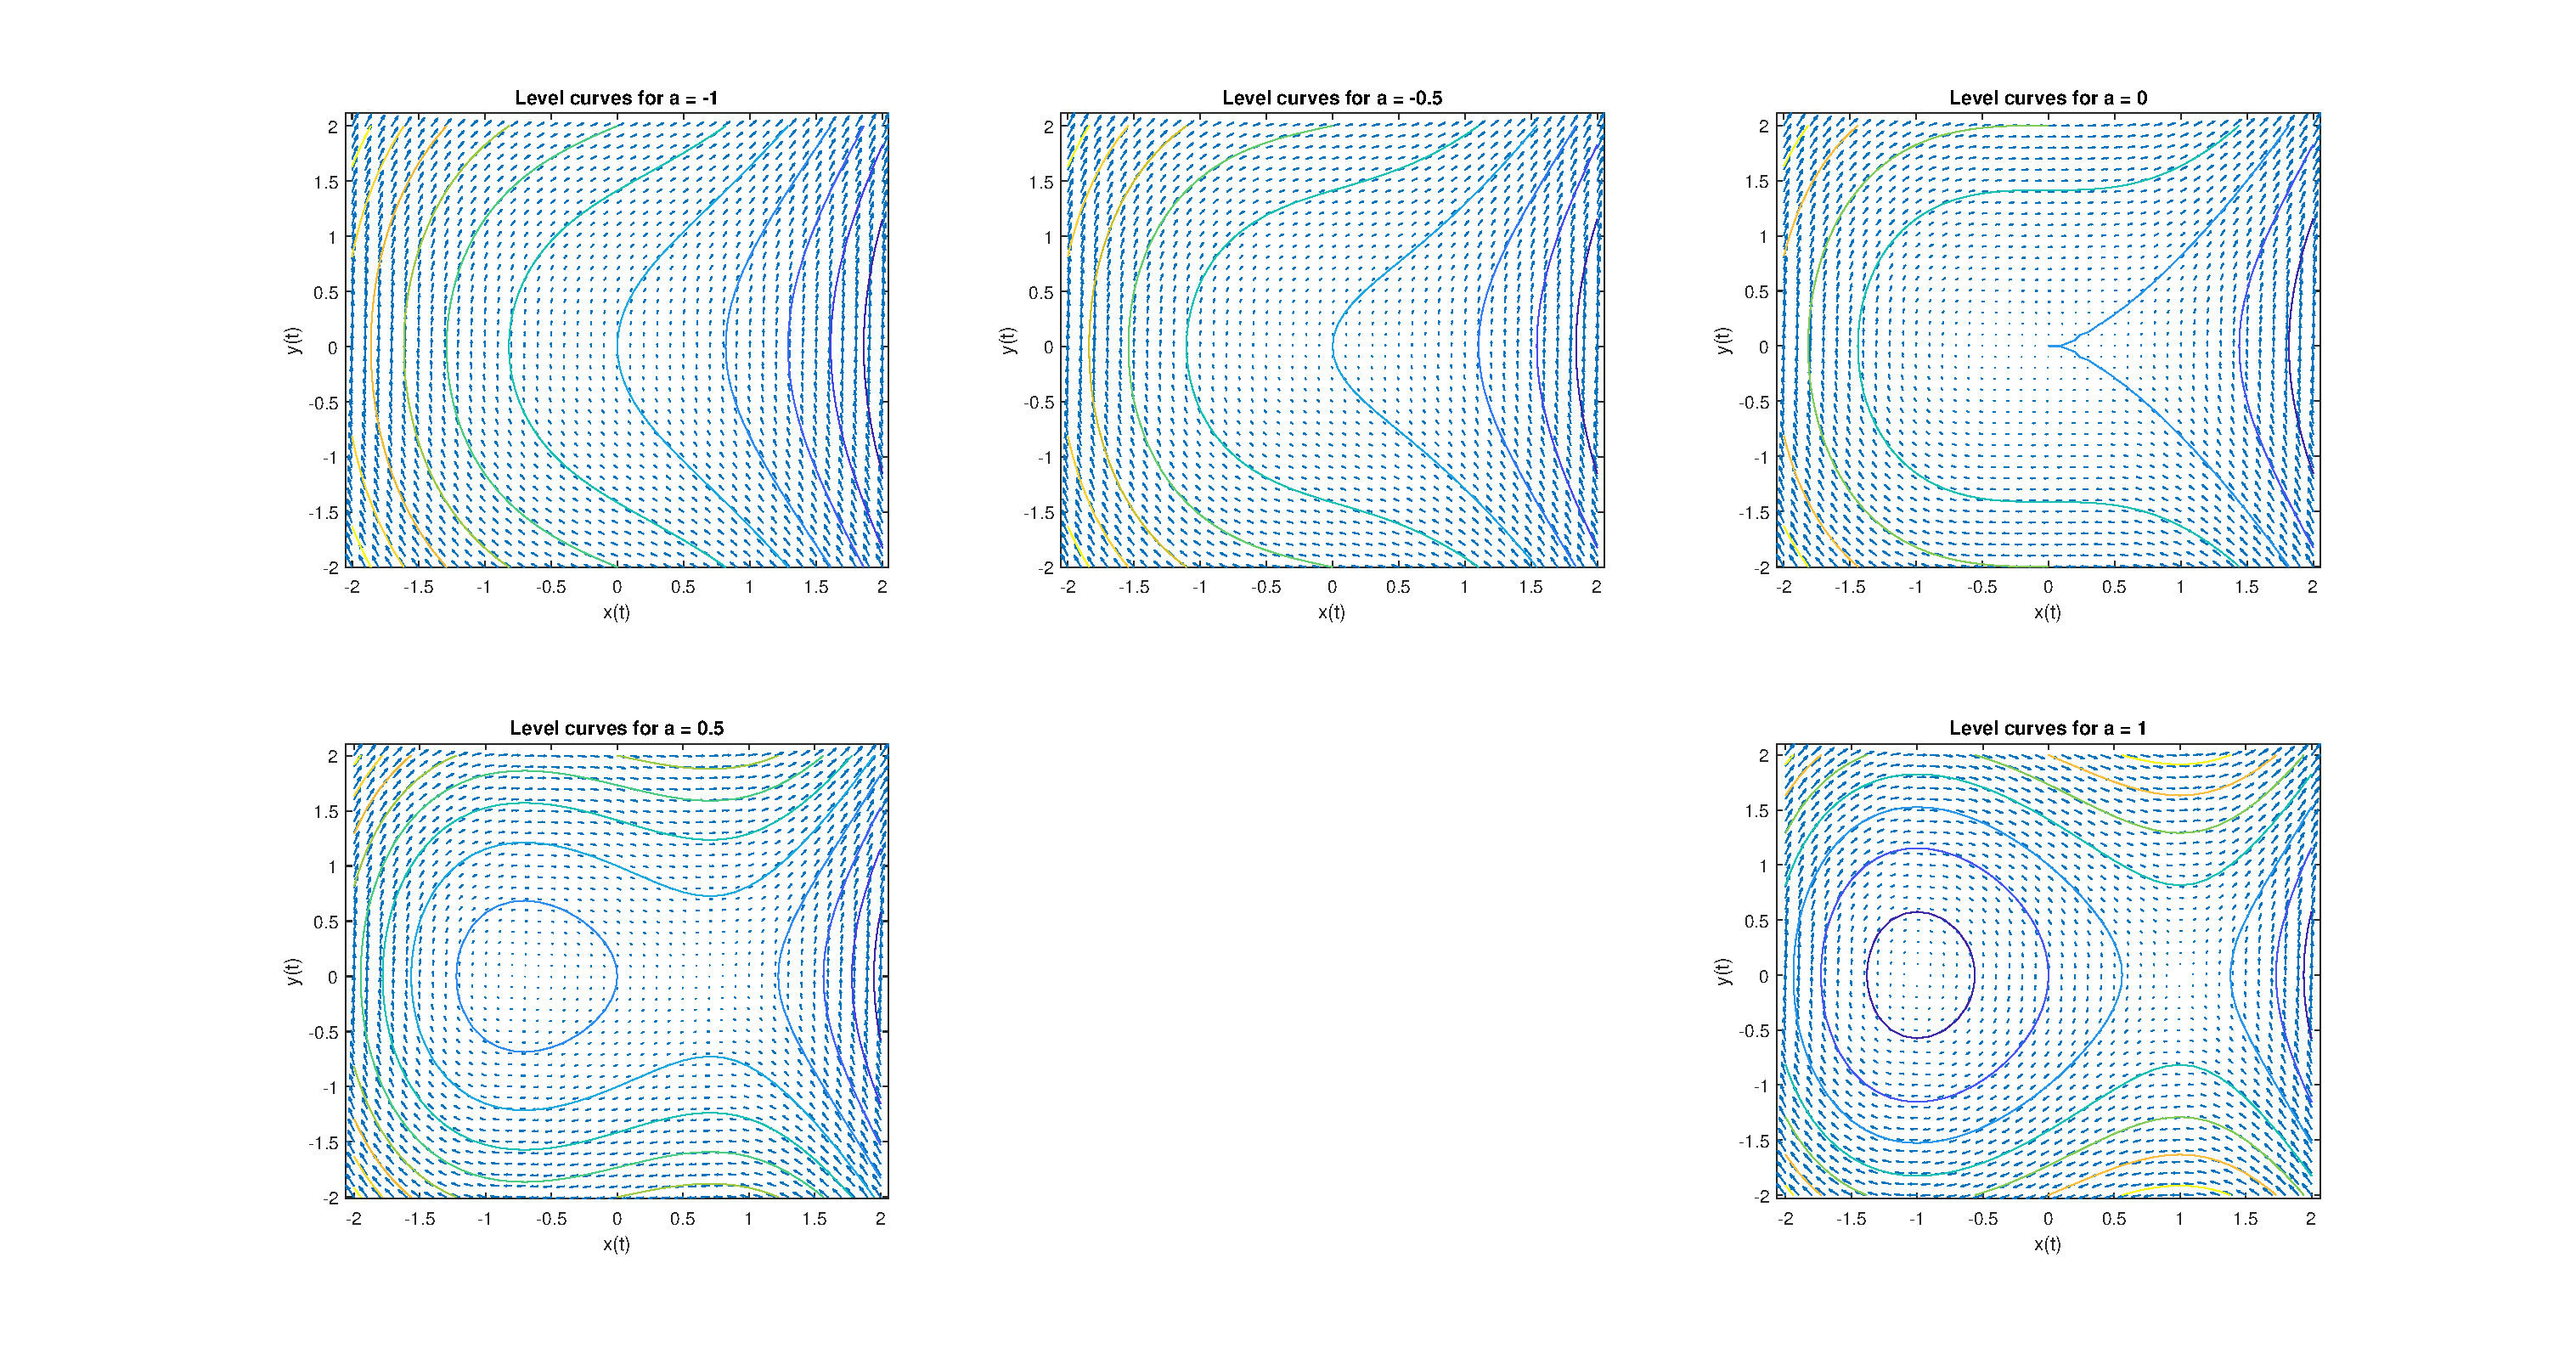
\includegraphics[trim={2in 0 1.5in 0}, width=\linewidth]{Figures/hamiltonian}
	\caption{Phase portrait of $H(x,y)$}
	\label{fig:hamiltonian}
\end{figure}



\end{Example}
\section{Dissipative Systems}
\section{Appendix}
\lstinputlisting{numerical_soln.m}
\bibliography{citations}
\bibliographystyle{plain}

\end{document}
